\documentclass[11pt,letterpaper]{article}
\usepackage[margin=1in]{geometry}
\usepackage[T1]{fontenc}
\usepackage{lmodern}
\usepackage{amsmath,amssymb,amsthm,mathtools}
\usepackage{microtype,booktabs,array,enumitem,graphicx}
\usepackage[dvipsnames]{xcolor}
\usepackage{fancyhdr}
\usepackage{xurl}
\usepackage{tocloft}
\setlength{\cftbeforesecskip}{2pt}
\usepackage[colorlinks=true,linkcolor=MidnightBlue,citecolor=MidnightBlue,urlcolor=MidnightBlue]{hyperref}
\newtheorem{theorem}{Theorem}[section]
\newtheorem{corollary}[theorem]{Corollary}
\newtheorem{proposition}[theorem]{Proposition}
\newtheorem{lemma}[theorem]{Lemma}
\theoremstyle{definition}
\newtheorem{definition}[theorem]{Definition}
\theoremstyle{remark}
\newtheorem{remark}[theorem]{Remark}
\newcommand{\Qp}{\mathbb Q_p}
\newcommand{\Zp}{\mathbb Z_p}
\newcommand{\Fp}{\mathbb F_p}
\setlength{\parskip}{4pt}
\setlength{\parindent}{0pt}
\setlength{\emergencystretch}{2em}
\pagestyle{fancy}
\fancyhf{}
\fancyhead[L]{\small ProveIt research extension}
\fancyhead[R]{\small November 27, 2026}
\fancyfoot[C]{\thepage}
\setlength{\headheight}{14pt}


\hypersetup{pdftitle={Exact exponent compression and deep p-adic roots},pdfauthor={Research prepared for Vladimir Reshetnikov}}
\title{Exact Exponent Compression\\and Deep $p$-adic Roots}
\author{Research prepared for Vladimir Reshetnikov\\\small An extension of the ProveIt GRH research programme}
\date{November 27, 2026}
\begin{document}
\maketitle
\begin{abstract}
We construct an invertible rational linear map between spaces of sparse
polynomials whose exponents agree to an explicit finite $p$-adic precision.
The map matches the first $t$ Euler derivatives and preserves, simultaneously,
the entire multiset of geometric root depths above $1/(p-1)$. This holds for
every term count $t$, including the range beyond $p$ left open in the source
article. Canonical representatives give a degree bound independent of the
original exponents. Finite lattice formulas then compute the sharp maxima
in every deeper closed disk and in the open critical disk; full-support,
simple, rational witnesses attain the maxima. As a concrete sharp case,
we prove that an eight-term polynomial has at most nine roots in
$v_2(X-1)>1$, with an explicit squarefree witness. Two independent exact
computations check all 165 residue patterns in that classification. The
theorems are unconditional. They address an explicit research question in
the repository; no resolution of a prominent classical conjecture or
certification of publication priority is claimed.
\end{abstract}
{\setlength{\parskip}{0pt}\tableofcontents}
\clearpage
\section*{Reader's guide and status}
\addcontentsline{toc}{section}{Reader's guide and status}
The main contribution is Theorem~\ref{thm:transport}: an exact equivalence
between spaces of polynomials of potentially enormous degree and finite
canonical models that retain at most the same number of terms. A usual
$p$-adic root bound alone does not give such an equivalence. The coefficient
map, the finite residue precision, and preservation of every deep root
radius are the structural results proved here.

The source is the ProveIt directory
\texttt{Analysis/GeneralizedRiemannHypothesis}, inspected at commit
\texttt{cfab41369737c66ae520d179419509eb719367cd}. Its question
\texttt{smd:q:roots} asks for additional residue data and exact root counts
when the number of exponents exceeds $p$. The present work answers this
in the form of explicit finite data and exact algorithms, without giving
a closed formula for all global maxima. The nine-root theorem is a complete
particular global evaluation, not a search over a bounded original degree.

Throughout, roots lie in an algebraic closure of $\mathbb Q_p$ and counts
include multiplicity, unless distinctness is stated. In particular, the
nine roots in the explicit example have nonintegral depth $10/9$ and are
not asserted to belong to $\mathbb Q_2$. The main proof has been checked
independently within this research session, but has not been formalized
or compiled in Lean. The accompanying finite certificates are exact
integer and rational computations.

\section{Finite residue transport of deep root spectra}
Fix a prime $p$, write $v=v_p$ with $v(p)=1$, and put $r_0=1/(p-1)$.
All polynomial coefficients and roots may belong to arbitrary finite extensions
of $\mathbb Q_p$. Roots are counted with multiplicity. For $t\ge2$ define
\[
 D_p(t)=\max_{0\le i<t}S_p(i),\qquad
 A_p(t)=\left\lceil\frac{D_p(t)-1}{p-1}\right\rceil,\qquad P_p(t)=p^{A_p(t)},
\]
where $S_p(i)$ is the base-$p$ digit sum. Here $A_p(t)\ge0$; modulus one
is meaningful when $A_p(t)=0$.

\begin{theorem}[Exact transport of deep root radii]\label{thm:transport}
Let $E,F$ be two sets of $t$ distinct nonnegative integers whose residue
multisets modulo $p^{A_p(t)}$ agree. There is a unique invertible rational
linear map
\[
 \mathcal T_{E,F}:\operatorname{span}_{\mathbb Q}\{X^n:n\in E\}
 \longrightarrow\operatorname{span}_{\mathbb Q}\{X^n:n\in F\}
\]
that matches the first $t$ Euler derivatives at one:
\[
 ((X\,d/dX)^i\mathcal T_{E,F}f)(1)=((X\,d/dX)^if)(1)
 \quad(0\le i<t).
\]
For every nonzero $f$, after scalar extension this map preserves the entire multiset
\[
 \{v(\alpha-1):f(\alpha)=0,\ v(\alpha-1)>r_0\},
\]
with multiplicity and with $+\infty$ included when $\alpha=1$.
It consequently preserves the number of roots in every closed disk
$v(X-1)\ge r$, for every real $r>r_0$, and in the open disk
$v(X-1)>r_0$. The same assertion holds about any nonzero centre after
scaling the variable.

\end{theorem}
\begin{proof}
For $f=\sum_{n\in E}c_nX^n$ let
$M_i(f)=\sum_{n\in E}c_nn^i$, using $n^0=1$. The matrix
$(n^i)_{0\le i<t,n\in E}$ is an ordinary Vandermonde matrix and is
invertible over $\mathbb Q$. This defines $\mathcal T_{E,F}$ and its inverse.
The moment sequence satisfies the integral monic recurrence with
characteristic polynomial $\Phi_E(T)=\prod_{n\in E}(T-n)$.
Normalize $f$ by a nonzero scalar so that
$\min_{i<t}v(M_i(f))=0$. Then all moments of $f$ and $g=\mathcal T_{E,F}f$
are integral. The residue hypothesis gives
$\Phi_E\equiv\Phi_F\pmod{p^A}$, where $A=A_p(t)$.
Induction in the two recurrences, starting with the identical first $t$
terms, yields
\[
 M_k(f)-M_k(g)\in p^A\mathcal O\quad(k\ge0).
\]
This is also true for $A=0$ without a residue hypothesis.
For rational $r>r_0$ choose $b$ in a finite extension with $v(b)=r$ and
substitute $X=\exp(bY)$. The coefficient of $Y^k$ is $M_k b^k/k!$.
Set
\[
 w_r(k)=rk-v_p(k!)=(r-r_0)k+\frac{S_p(k)}{p-1},\qquad
 M_r=\max_{0\le i<t}w_r(i).
\]
Some initial moment is a unit, so the minimum coefficient valuation of
each series is at most $M_r$. For every $k\ge t$, the strict inequality
$i-k<0$ gives
\[
 M_r-w_r(k)
 =\max_{i<t}\left((r-r_0)(i-k)+\frac{S_p(i)-S_p(k)}{p-1}\right)
 <\frac{D_p(t)-1}{p-1}\le A.
\]
Hence the difference of the two coefficients at $k\ge t$ has valuation
at least $A+w_r(k)>M_r$; the initial coefficients are identical.
The two coefficient sequences therefore have identical valuations at
every index whose valuation is at most $M_r$, and in particular have
the same minimum and the same minimizing indices.
The series are restricted power series because $w_r(k)\to\infty$.
By the Newton polygon/Weierstrass rule their largest minimizing indices
count roots in the closed unit disk. The exponential substitution is a
bijection onto $v(X-1)\ge r$ with nonzero derivative, so multiplicities
are preserved. This proves equality at every rational $r>r_0$.
Algebraic root valuations are rational (apart from $+\infty$), and each
polynomial has finitely many roots, so the equality of all these counting
functions proves equality of the complete multisets. In particular it
also proves the claim at irrational radii and in the open disk.\end{proof}

\paragraph{What the theorem does and does not preserve.}
The map matches a finite Euler jet and preserves root depths. It need
not preserve individual root locations, their residue fields, their
Galois orbits, or whether roots lie in one prescribed local field.
Coefficients are changed by the map; exponents cannot simply be reduced
while leaving coefficients fixed. The theorem concerns geometric roots
in the algebraic closure in one sufficiently deep disk.

\section{Canonical bounded-degree reduction}
For the residue multiplicities $\nu_c$ modulo $P=P_p(t)$ define
\[
 E_\nu=\{c+jP:0\le c<P,\ 0\le j<\nu_c\},\qquad \sum_c\nu_c=t.
\]
Transport to this support, then factor out its smallest monomial.
The resulting polynomial has degree at most $(t-1)P$. Indeed if a single
residue occurs, its exponent diameter is exactly $(t-1)P$. Otherwise
all multiplicities are at most $t-1$, and the diameter is at most
$(t-2)P+(P-1)=(t-1)P-1$. Factoring out a monomial changes no root in the
disk about one. Thus every polynomial with at most $t$ terms has at most
\[
 (t-1)p^{A_p(t)}
\]
roots in $v(X-1)>1/(p-1)$, counted with multiplicity, and the complete
deep-root spectrum can be realized by a polynomial of this bounded
degree. Pad a support with zero coefficients if it has fewer than $t$
terms. More importantly, the exact fixed-support extremum and the global
extremum are finite computable problems for every $p,t$ and every rational
closed-disk depth $r>r_0$, as well as in the open critical disk:
there are only $\binom{P+t-1}{t}$ residue multisets.

\section{Exact finite lattice rules for open and closed disks}
Let $E=\{n_1,\ldots,n_t\}$ be any fixed finite support, put $d=\max E$, and
write $a_k=(\binom{n_j}{k})_{j=1}^t\in\mathbb Z^t$ for $0\le k\le d$,
using zero binomial coefficients when $k>n_j$.
For rational $r=a/e>0$ in lowest terms let $\pi^e=p$,
$K=\mathbb Q_p(\pi)$, and $\mathcal O=\mathbb Z_p[\pi]$. Define
\[
 v_k=\pi^{ak}a_k,\qquad L_r=\sum_{k=0}^d\mathcal O v_k\subset K^t.
\]
This is a full lattice: the polynomials $(1+Y)^{n_j}$ are linearly
independent, so the Taylor row vectors span $K^t$.

\paragraph{Closed disk rule.}
The maximum number of geometric roots of a nonzero polynomial supported
on $E$ in $v(X-1)\ge r$, counted with multiplicity, is exactly
\[
 C_E(r)=\max\{k:v_k\notin\pi L_r\}.
\]
For the upper bound, normalize the coefficient functional so that its
minimum value on the generating columns has valuation zero. It is then
integral on $L_r$, and takes every vector of $\pi L_r$ to an element of
positive valuation. Thus the last minimizing index is at most the
displayed maximum. For the lower bound, a nonzero class of $v_k$ in
$L_r/\pi L_r$ admits an $\mathbb F_p$-linear functional taking it to one.
Lift this functional to $\operatorname{Hom}_{\mathcal O}(L_r,\mathcal O)$.
If $k$ is the largest such index, all later generators have zero
reduction, so $k$ is precisely the last minimizing index. Newton's rule
proves attainment. The argument works equally for coefficient fields
extending $K$, and shows that such extensions cannot improve the bound.

\paragraph{Open disk rule.}
For $r=r_0=1/(p-1)$ take $e=p-1$, $a=1$ and the same finite Taylor lattice
$L=L_{r_0}$. Write $\bar v_k$ for the images in $L/\pi L$. Then the sharp
count in $v(X-1)>r_0$ is
\[
 O_E=\max\{k:\bar v_k\notin
   \operatorname{span}_{\mathbb F_p}(\bar v_0,\ldots,\bar v_{k-1})\}.
\]
Here the smallest minimizing coefficient index counts roots strictly
inside the unit disk. A normalized coefficient functional has that
smallest index equal to $k$ exactly when its reduction annihilates all
earlier columns but not $\bar v_k$. Such a functional exists exactly
when the displayed span condition holds. This is the last rank-increase
index of the ordered columns. It is essential to use the prefix span:
the simpler primitive-column rule answers the closed disk question.
For coefficients in a further finite extension $H/K$, reduce the normalized
functional modulo the maximal ideal of $\mathcal O_H$, into its residue
field. It still kills $\pi L$
and is $\mathbb F_p$-linear on $L/\pi L$. If $\bar v_k$ lies in the
earlier span, it therefore cannot be the first nonzero image. Conversely,
an $\mathbb F_p$-valued separating functional already supplies a witness
over $K$. Thus arbitrary ramification does not change this maximum.

\paragraph{Exact computation.}
Represent $\mathcal O^t$ as the free $\mathbb Z_p$-module with basis
$\pi^z e_i$, $0\le z<e$, $1\le i\le t$. Each lattice generator and its
$\pi^z$ multiples then has integer coordinates, since $\pi^e=p$.
Integer Hermite normal form computes a basis after localization at $p$.
Membership in $\pi L$ is exact rational linear algebra followed by
$p$-adic valuation comparisons. The open rule can alternatively be
computed from the determinant-index drops upon successively adjoining
$v_0,v_1,\ldots$ to $\pi L$. Every index drop is zero or one in valuation,
since the quotient is an $\mathbb F_p$ vector space and one vector is
adjoined at a time. This uses no floating point arithmetic.

\paragraph{A determinant formula for the whole depth profile.}
There is also a finite expression without a choice of lattice basis.
Let $\mathcal B$ be the collection of $t$-element subsets of
$\{0,\ldots,d\}$ for which the matrix with columns $a_k$, $k\in B$,
has nonzero determinant $\Delta_B$. Define
\[
 h_B(r)=v_p(\Delta_B)+r\sum_{k\in B}k,
 \qquad \mathcal B_r=\operatorname*{arg\,min}_{B\in\mathcal B}h_B(r).
\]
For rational $r>0$, the minimal determinant valuation is the valuation
of the determinant of $L_r$. The minimizing subsets are exactly the
bases of $L_r$ chosen from its generating columns. A column is primitive
if and only if it belongs to one of those bases, because its nonzero
reduction can be extended to a basis using the other generating columns.
The first prefix spanning $L_r/\pi L_r$ is the first prefix containing
such a basis. Consequently
\[
 C_E(r)=\max_{B\in\mathcal B_r}\max B,
 \qquad O_E=\min_{B\in\mathcal B_{r_0}}\max B.
\]
The lower envelope of the finitely many affine functions $h_B$ has
rational breakpoints. Thus the closed-count function is specified on
every real depth by finitely many rational intervals and their endpoints;
at irrational depths the formula follows from any rational depth in the
same interval. This supplies an exact finite description of the whole
depth profile, although direct enumeration of all minors can be costly.

\section{Rational, simple, full-support witnesses}
The extremal counts in both rules are attained by integer polynomials
with every allowed exponent present and with every root in the disk
simple. After removal of a common monomial one may also require
irreducibility over $\mathbb Q$. Remove that monomial first, which
preserves all counts in the disk and ensures that exponent zero is allowed.
First the dual-lattice argument provides a coefficient vector over
$K=\mathbb Q_p(\pi)$. Express it as
$c=\sum_{z=0}^{e-1}\pi^z c_z$, where $c_z\in\mathbb Q_p^t$.
For every Taylor coefficient the terms in this expansion have distinct
valuations modulo $\mathbb Z$, so their sum has valuation equal to the
minimum of their valuations. Choose a component attaining the relevant
minimum at the desired index. For the closed rule, all later indices
are strictly larger in the original vector, hence also in that
component; for the open rule all earlier indices are strictly larger.
The chosen $\mathbb Q_p$ component therefore attains the same extremal
index. Approximate its coefficients by rational numbers closely enough
to preserve the finite coefficient-valuation comparisons. After
clearing denominators, arbitrarily small perturbations by large powers
of $p$ make every allowed coefficient nonzero. Choose another prime
$q\ne p$ not dividing the leading coefficient. By the Chinese remainder
theorem these perturbations can simultaneously impose Eisenstein
congruences at $q$: all nonleading coefficients divisible by $q$, and
the constant coefficient divisible by $q$ but not $q^2$. Missing
coefficients already vanish and satisfy the required divisibility.
This gives an irreducible polynomial in characteristic zero, hence
simple roots, while preserving the relevant deep-disk count.

\section{Higher residue precision is necessary}
At $p=2,t=8$, one has $D_2(8)=3$ and $A_2(8)=2$.
The supports
\[
 E=\{0,1,2,3,4,5,6,7\},\qquad
 F=\{0,1,2,3,4,5,7,8\}
\]
have identical residue multiplicities modulo two: four even and four
odd exponents. The first has sharp open-disk count seven by its degree,
attained by seven distinct integer roots congruent to one modulo four.
The second has sharp count eight, also by its degree, attained by
\[
 Q(X)=(X-1)^7(X+3)+2^{11}.
\]
The coefficient of $X^6$ is zero and all eight other coefficients are
nonzero:
\[
 Q(X)=X^8-4X^7+28X^5-70X^4+84X^3-56X^2+20X+2045.
\]
After $X=1+Y$ it is $Y^8+4Y^7+2^{11}$. Its Newton polygon has a single
segment from $(0,11)$ to $(8,0)$; the point $(7,2)$ is strictly above it.
All eight roots consequently have valuation $v_2(X-1)=11/8$.
Its derivative in $Y$ is $4Y^6(2Y+7)$, and neither zero nor $-7/2$ is a
root of the polynomial, proving squarefreeness directly. The same
example distinguishes the closed-disk counts at depth $5/4$.
Thus reduction modulo two cannot determine these extrema; the higher
residue information in the main theorem is genuinely needed.

\section{Exact eight-term maximum in the deep two-adic disk}
Let $N_p^\circ(t)$ denote the maximum number of geometric roots in
$v_p(X-1)>1/(p-1)$ among nonzero polynomials with at most $t$ nonzero
terms, allowing coefficients in any finite extension of $\mathbb Q_p$.
Let $N_p^\circ(E)$ denote the corresponding maximum for a fixed allowed
support $E$. The preceding witness argument shows that these maxima
are unchanged if one requires integer coefficients and simple roots
in the disk.

\begin{theorem}[Exact eight-term classification]\label{thm:eight}
For an eight-element support $E$, let $\nu_c$ be the number of its
exponents congruent to $c$ modulo four, and put $e=\nu_0+\nu_2$. Then
\[
 N_2^\circ(E)=
 \begin{cases}
 9,&e\equiv2\pmod4,\\
 7,&e\equiv0\pmod4\text{ and all four }\nu_c\text{ have the same parity},\\
 8,&\text{otherwise}.
 \end{cases}
\]
Consequently
\[
 N_2^{\circ}(8)=9.
\]
\end{theorem}
\begin{proof}[Finite certificate proof of the upper bound and classification]
The transport theorem reduces all supports to the $\binom{11}{3}=165$
residue multiplicity vectors modulo four. The finite Taylor lattice
criterion gives maxima seven for 23 vectors, eight for 100 vectors,
and nine for 42 vectors. Two independent exact implementations agree on every case. The certificate records each canonical
support, each lattice basis, its determinant valuation, and every
prefix rank increment. The generator is exact integer/rational
arithmetic and the independent checker verifies the same classification by rational elimination over the local ring $\mathbb Z_{(2)}$, without Hermite normal form.
This exact classification is a finite computer-assisted theorem;
it is separate from the purely symbolic transport proof.
The compact formula in Theorem~\ref{thm:eight} is checked against every
profile. The lattice witness theorem proves that each fixed-support
maximum is attained, including with every allowed coefficient nonzero.
Supports with fewer than eight exponents can be padded with zero
coefficients, so the bound nine also applies to the at-most-eight class.
\end{proof}

Sharpness also has a short explicit witness:
\[
 P(X)=183X^{10}-235X^8+54X^6-6X^4-128X^3+3X^2+128X+2049.
\]
It has eight terms, and
\begin{align*}
 P(1+Y)={}&183Y^{10}+1830Y^9+8000Y^8+20080Y^7+31904Y^6\\
 &+33280Y^5+22784Y^4+9728Y^3+2048Y^2+2048.
\end{align*}
The lower Newton polygon has vertices $(0,11),(9,1),(10,0)$.
It has nine roots of valuation $10/9$ and one of valuation one.
An exact Euclidean gcd calculation gives $\gcd(P,P')=1$.
There is also a small independent certificate modulo seven: with
\begin{align*}
 A(X)&=3X^8-X^6-X^5-3X^4+3X^3-X^2+3X-1,\\
 B(X)&=-X^9+3X^7-2X^6-3X^5+2X^4-3X^3-3X^2+2X+3,
\end{align*}
one has $AP+BP'\equiv1\pmod7$. Since the leading coefficient of
$P$ is nonzero modulo seven, this also proves squarefreeness over
$\mathbb Q$.
The nine deep roots are therefore distinct. Figure~\ref{fig:newton} displays the exact Newton polygon.
\begin{figure}[ht]
\centering
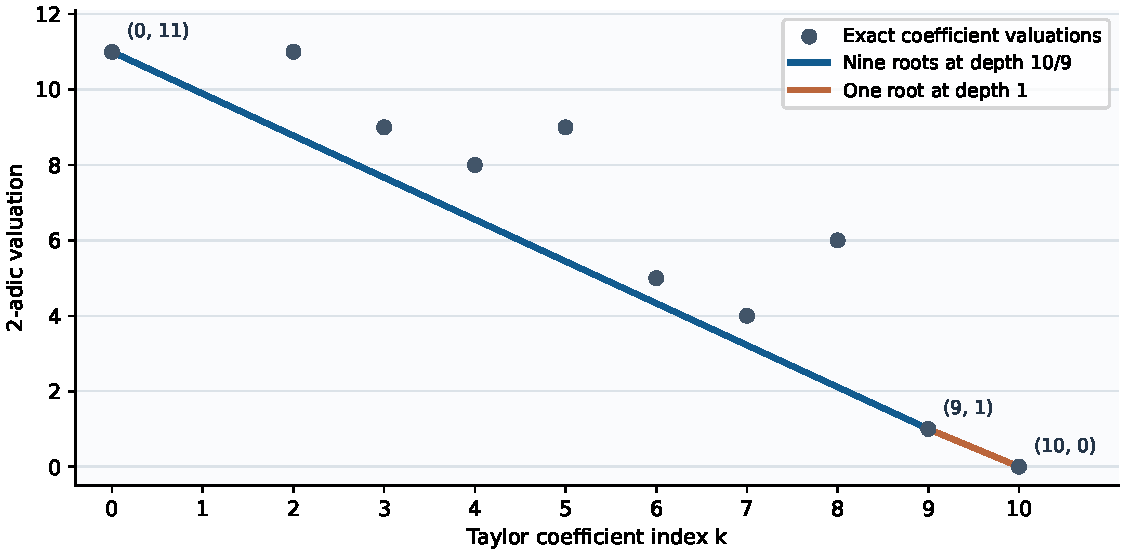
\includegraphics[width=.92\linewidth]{figures/nine_roots_newton.pdf}
\caption{The lower Newton polygon of $P(1+Y)$. The first segment has horizontal length nine and slope $-10/9$; the last root lies on the excluded boundary of depth one. No numerical root approximation is used.}\label{fig:newton}
\end{figure}

\section{Scope and relation to the repository}\label{sec:scope}
At the pinned revision \cite{ProveIt}, the source article's Question \texttt{smd:q:roots} asks which additional
residue data determine exact root counts beyond $p$ terms, both in the
open disk and on deeper closed disks. Its rank rule was restricted to
at most $p$ exponents, with separate $p+1,p+2$ open maxima. The transport
and finite lattice rules answer the finite-data and exact-computability
question for arbitrary term count and every depth. They do not supply
a closed formula in $p,t$ for every global maximum, and do not prove the
singular-modulus six-term conjecture. They are independent of RH and
Dirichlet GRH, although the source question arose in the repository's broader
GRH-driven research programme. A claim of global publication priority
requires further literature review; this is a proved new extension of
the inspected repository, not a claimed resolution of a famous general
fewnomial conjecture.

\section{Two strengthenings and a sharp boundary}
The moment proof only uses
\[
 \prod_{n\in E}(T-n)\equiv\prod_{m\in F}(T-m)\pmod{p^{A_p(t)}}.
\]
One may use this congruence of monic characteristic polynomials as the
hypothesis of the main theorem; equality of residue multisets is a
particularly transparent sufficient condition. The latter, rather than
an unproved optimal minimal modulus, gives the finite enumeration.

The strict depth restriction cannot be dropped. For $t=2$, the
first-two-moment transport sends $X^p-1$ to $p(X-1)$.
Both have exactly one root in $v(X-1)>1/(p-1)$, but on the closed boundary
disk the first has $p$ roots and the second has only one: the nontrivial
$p$th roots of unity have depth exactly $1/(p-1)$.

A further corollary covers confluent exponential sums
\[
 F(u)=\sum_{j=1}^s P_j(u)e^{\alpha_j u},\qquad
 \alpha_j\in\mathbb Z_p,\quad \deg P_j<m_j,\quad t=\sum_jm_j.
\]
Here $F$ is nonzero, the $m_j$ are positive integers, and $t\ge2$.
For pairwise distinct $\alpha_j$ the first $t$ derivatives determine $F$ by the
confluent Vandermonde determinant. Its derivative sequence satisfies
the monic integral recurrence with characteristic polynomial
$\prod_j(T-\alpha_j)^{m_j}$. Replace the frequencies, with multiplicity,
by distinct canonical nonnegative integers having the same residues
modulo $p^{A_p(t)}$, and match the first $t$ derivatives with
$G(e^u)$, where $G$ is supported on those canonical exponents.
Exactly the same recurrence and weight argument shows that $F$ and
$G(e^u)$ have identical root valuation multisets in $v(u)>1/(p-1)$.
Here $v(e^u-1)=v(u)$ in the domain of the exponential, so the canonical
degree bound also applies to these confluent sums. This corollary needs
no extra asymptotic estimate or zero-distribution hypothesis.



\section{Initial forms and an effective implementation}
The proof gives slightly more than equality of counts. At any rational
$r>1/(p-1)$, after the common moment normalization and the substitution
$X=\exp(bY)$, the two series differ in every coefficient by a quantity of
valuation strictly greater than the common minimum. Divide both by a
coefficient attaining that minimum. Their reductions are then identical
polynomials over the residue field. Thus the exact transfer preserves
the initial polynomial at every deep radius, as well as the radial Newton
data. At a fixed depth $r$, the nonzero roots of this reduced polynomial
record, with multiplicity, the leading residue of $(\alpha-1)/b$:
$\exp(bY)-1$ and $bY$ have the same leading term. Hence the deep roots
can be paired, with multiplicity, so that for each pair different from one,
\[
 v_p(\alpha-\beta)>v_p(\alpha-1)=v_p(\beta-1).
\]
Roots at one are paired separately; their multiplicity is the first
nonzero moment index, which is below $t$ and is exactly preserved.
This is a statement about the first residue at each depth. It does not
assert equality of individual roots, higher cluster geometry, or fields
of definition.

For a specified rational input polynomial, the transport can be computed
by forming its first $t$ moments and solving one rational Vandermonde
system on the canonical support. Expand the resulting bounded-degree
polynomial at $X=1$, compute its coefficient valuations exactly, and take
the lower Newton polygon. Retain its segments of slope less than
$-1/(p-1)$ and record the horizontal lengths. The initial zero coefficients
record the multiplicity at $X=1$.

For fixed $p$, this procedure takes polynomial time in the sparse binary
input size. Indeed, if $h=\lfloor\log_p(t-1)\rfloor$, then
$D_p(t)\le(p-1)(h+1)$, so
$P_p(t)\le p^{h+1}\le p(t-1)$ and the degree span is at most
$p(t-1)^2$. The moments use powers of order below $t$, hence have
polynomial bit length; rational elimination and the subsequent dense
translation also have polynomial bit complexity. If $p$ varies, this
bound is polynomial in $p$, not in $\log p$. The complexity statement
is a consequence of this construction, not a claim of the first
polynomial-time geometric profile algorithm: classical finite root
bounds also permit a dense Taylor truncation approach.

\section{Prior work, novelty, and remaining questions}
Lenstra's fewnomial work already proves degree-independent bounds for
geometric roots in positive-depth disks, and explicitly discusses the
factorial method in the exponential convergence range \cite{Lenstra}.
Avenda\~no and Krick study sharp bounds for roots in fixed local fields,
with hypotheses involving ramification, residue degree, and term count
\cite{AvendanoKrick}. Rojas and Zhu give algorithms and separation bounds
for very sparse polynomials over $p$-adic fields \cite{RojasZhu}. These
are important precedents. Finiteness itself, the Newton polygon rule,
and linear recurrence arguments are not claimed as new.

The new assertions relative to the inspected source article are the
explicit support-space isomorphism, its uniform residue precision for
arbitrary $t$, its simultaneous preservation of every deep radius,
the finite classification of exact extrema, and the evaluation
$N_2^\circ(8)=9$. Targeted searches in the primary literature did not
locate these exact statements. Such searches do not establish global
publication priority. In particular, this work does not compute the
optimal number of roots in a prescribed finite extension of $\mathbb Q_p$:
the transfer need not preserve splitting fields. It also does not settle
the six-term singular-modulus question in the repository, or a general
fewnomial conjecture. The explicit uniform modulus is sufficient; its
minimality for arbitrary $(p,t)$ remains open.

\section{Reproduction and formalization boundary}
The archive contains two independent implementations of the eight-term
classification. The Hermite-normal-form computation in
\texttt{checks/exact\_lattice\_check.py} uses SymPy over exact integers and
rationals. The computation in \texttt{checks/independent\_dvr\_check.py}
uses only Python's standard library and valuation-minimal pivots over
$\mathbb Z_{(2)}$. They agree on every one of the 165 residue vectors.
Both outputs give the distribution $(23,100,42)$ of maxima $(7,8,9)$.
The first output retains full HNF bases and prefix-index drops; the second
retains the independent pivot data.

An additional standard-library checker compares complete Newton polygons
before and after the rational moment map in 256 deterministic cases,
using $p=2,3,5,7$ and $2\le t\le9$. It also includes cases with more
than $t-1$ deep roots. These examples test the implementation; the
general theorem is established by the recurrence and strict-weight proof,
not by sampling. The explicit eight- and nine-root witnesses are checked
by exact expansions, coefficient valuations, and polynomial gcds.

The file \texttt{FORMALIZATION.md} separates finite algebra, valuation
estimates, the analytic Newton--Weierstrass bridge, and the finite
certificate theorem into suggested formalization units. No new result
in this archive is represented as Lean-kernel checked.

\begin{thebibliography}{9}
\bibitem{ProveIt} V. Reshetnikov, \emph{ProveIt: Beyond the Riemann hypothesis
for Dirichlet $L$-functions}, pinned revision
\texttt{cfab41369737c66ae520d179419509eb719367cd}, section on sparse equations
for singular moduli, especially \texttt{smd:thm:rankrule} and
\texttt{smd:q:roots}.\newline
\url{https://github.com/VladimirReshetnikov/ProveIt/blob/cfab41369737c66ae520d179419509eb719367cd/Analysis/GeneralizedRiemannHypothesis/Article/sections/smd.tex}.
\bibitem{Lenstra} H. W. Lenstra Jr., \emph{On the factorization of lacunary
polynomials}, Number Theory in Progress, vol. 1 (1999), 277--292.
\url{https://doi.org/10.1515/9783110285581.277}.
\bibitem{AvendanoKrick} M. Avenda\~no and T. Krick, \emph{Sharp bounds for the
number of roots of univariate fewnomials}, Journal of Number Theory
131 (2011), 1209--1228. \url{https://doi.org/10.1016/j.jnt.2011.01.006}.
\bibitem{RojasZhu} J. M. Rojas and Y. Zhu, \emph{Root repulsion and faster
solving for very sparse polynomials over $p$-adic fields}, preprint
arXiv:2107.09173 (2021). \url{https://arxiv.org/abs/2107.09173}.
\end{thebibliography}
\end{document}

